\begin{figure}
	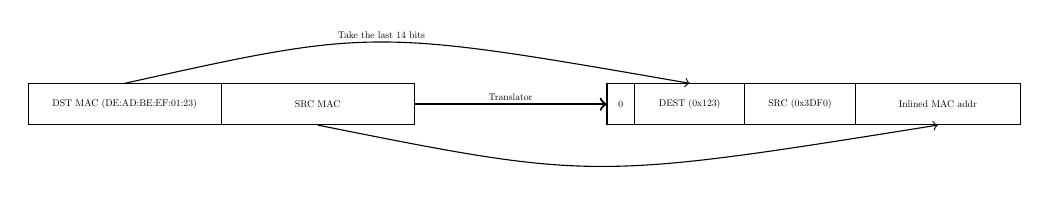
\begin{tikzpicture}[scale=0.35,  every node/.style={scale=0.35},
		region/.style={
			rectangle,
			draw,
			minimum height=1.5cm}]

		\node (dstmac) [region,, minimum width=7cm] {DST MAC (DE:AD:BE:EF:01:23)};
		\node (srcmac) [region, right of=dstmac, xshift=6cm, minimum width=7cm] {SRC MAC};

		\node (mcast) [region,right of=srcmac, xshift=10cm, minimum width=1cm] {0};
		\node (dest) [region, right of=mcast,xshift=1.5cm, minimum width=4cm] {DEST (0x123)};
		\node (src) [region, right of=dest,xshift=3cm, minimum width=4cm] {SRC (0x3DF0)};
		\node (dstmacil) [region, right of=src,xshift=4cm, minimum width=6cm] {Inlined MAC addr};

		\draw[thick, ->] (srcmac.east) -- (mcast.west) node [midway, above] {Translator};
		\draw[->] (srcmac.south) .. controls ++(10cm,-2cm) .. (dstmacil.south);
		\draw[->] (dstmac.north) .. controls ++(9cm,2cm) .. (dest.north) node [midway, above] {Take the last 14 bits};
	\end{tikzpicture}
\end{figure}